\chapter{Trabalhos Relacionados} 
\label{chap:trab_relacionados}

% Neste capítulo serão apresentados trabalhos correlatos a este em ordem cronológica de
% publicação. Cada seção é referente a um tópico desta pesquisa, sendo as duas primeiras (Seções
% 3.1 e 3.2), segmentação e classificação, relacionadas a tarefas de visão computacional e divididas entre trabalhos envolvendo a criação de bases de dados (Seções 3.1.1 e 3.2.1) e de modelos
% (Seções 3.1.2 e 3.2.2) para cada um dos tópicos em questão. A Seção 3.3, reconhecimento automático de dor em recém-nascidos, traz algumas das abordagens criadas em função dos anos,
% para contextualização sobre as técnica disponíveis no meio.

Aplicar a unificação de técnicas radiômicas e \textit{deeplearning} em cardiomiopatias já são objeto de estudo em diversas pesquisas recentes.
Neste capítulo serão apresentados trabalhos e metodologias correlatos ao esforço de outros autores a cerca deste tema. As seções se referem a um tópico ou metodologia aplicados nesta pesquisa sendo a primeira (Seção \ref{sec:rev_sistematica}) responsável pela revisão sistemática da literatura.

%---------------------------------------------------------
\section{Revisão Sistemática da Literatura} 
\label{sec:rev_sistematica}

Para a fase exploratória dos trabalhos relacionados, foi utilizada a ferramenta \textit{Parsifal} com o objetivo de identificar estudos onde se aplica a análise radiômica no contexto de cardiopatia. O objetivo inicialmente definido foi o seguinte: "Identificar estudos onde se aplica análise radiômica a cardiopatia. Em segunda opção, alguma outra doença de natureza cardíaca". A pesquisa teve como objetivo responder as seguintes perguntas: quais desafios descritos nos estudos prévios e se há replicabilidade da proposta. As palavras chaves selecionadas são: \textit{cardiac}, \textit{cardiomyopathy} e \textit{radiomics}. A palavra de busca selecionada foi: ``\textit{radiomics} AND (\textit{cardiac} OR \textit{cardiomyopathy})'' com o intuito de filtrar os resultados de forma a identificar onde na ciência poderia identificar a interseção de ambas as abordagens(radiômica e \textit{deep}). Os resultado da busca pode ser conferido na Tabela \ref{tab:resultado_busca}. 

\begin{table}[hbtp]
    \centering
    \renewcommand{\arraystretch}{1.4} % default é 1 
    \begin{tabular}{|c|c|}
    \hline 
          \textbf{Origem} & \textbf{Artigos}  \\ 
    \hline 
        IEEE & 6 \\ 
        PUBMED & 19 \\ 
        Science@Direct & 24 \\ 
    \hline 
    \end{tabular} 
    \caption{Resultados dos Artigos}
    \label{tab:resultado_busca}
\end{table}

Em posse dos resultados, alguns critérios de aceitação foram aplicados como pode ser visto na Tabela \ref{tab:criterios}).

\begin{table}[hbtp]
    \centering
    \caption{Critérios de Inclusão e Exclusão}
    \renewcommand{\arraystretch}{1.4} % default é 1 
    \begin{tabular}{|l|l|}
    \hline 
          \multicolumn{1}{|c|}{\textbf{Critério de Inclusão}} & \multicolumn{1}{c|}{\textbf{Critério de Exclusão}}  \\ 
    \hline 
        \quad Contém ressonância magnética? & \quad Estudos Duplicados   \\ 
        \quad O objeto de estudo é o coração? & \quad Estudos Secundários ou Terciários \\
        \quad Usa análise de textura? & \quad Estudos que não estão em PT ou EN\\
        \quad Utiliza análise radiômica? & \quad Leitura cinza  \\
        \quad É cardiomiopatia? & \quad Não aplica técnicas computacionais\\
        & \quad Não trata do coração \\
        & \quad Não usa RM \\
        & \quad Trabalho que atua somente com dados genômicos \\ 
    \hline 
    \end{tabular} 
    \caption*{Fonte: Autor}
    \label{tab:criterios}
\end{table}

Critérios de aceitação também foram aplicados e podem ser conferidos na Tabela \ref{tab:questoes}. Dentre cada uma das seis perguntas, calculamos a nota usando como pontuação 1 para sim, 0,5 para parcial e 0 para talvez. Como nota de corte usamos o valor 3, ou seja, qualquer artigo que não alcance o valor mínimo de 3, é descartado. Uma vez aplicado os critérios de aceitação, restaram 18 artigos dos 49 artigos iniciais.

\begin{table}[hbtp]
    \centering
    \renewcommand{\arraystretch}{1.4} % default é 1 
    \begin{tabular}{|l|}
    \hline 
          \multicolumn{1}{|c|}{\textbf{Questões}} \\ 
    \hline 
        \quad É descrita as limitações do estudo? \\
        \quad Há um experimento bem descrito para avaliar a proposta? \\
        \quad Há mais de 2 autores? \\
        \quad O trabalho apresenta resultados? \\
        \quad A introdução apresenta o problema de forma clara \\
        \quad É análise sistemática da literatura? \\
    \hline 
    \end{tabular} 
    \caption{Questões de Aceitação}
    \label{tab:questoes}
\end{table}

%---------------------------------------------------------
\section{Análise Radiômica com Atenção}
\label{sec:analise_radiomica}

 \citeauthor{jiangMRIBasedRadiomics2021} \citeyear{jiangMRIBasedRadiomics2021} conduziram um estudo abrangente que aproveita as capacidades do aprendizado de máquina para melhorar os processos diagnósticos em oncologia, especificamente focando no câncer de colo de útero em estágio inicial. Sua pesquisa, intitulada "Abordagem Radiômica Baseada em Ressonância Magnética com Aprendizado Profundo para Predição de Invasão Vascular em Câncer de Colo de Útero em Estágio Inicial", foca na aplicação de técnicas de aprendizado profundo em dados de ressonância magnética multiparamétrica para prever a invasão vascular, um fator crítico para determinar a agressividade do câncer de colo de útero e informar estratégias de tratamento.

O estudo utilizou um conjunto substancial de dados compreendendo 1.070 imagens de ressonância magnética com contraste dinâmico T1 (DCE-T1) e 986 imagens de ressonância magnética ponderada em T2 (T2WI) coletadas de 167 pacientes diagnosticadas com câncer de colo de útero em estágio inicial entre janeiro de 2014 e agosto de 2018. Os pesquisadores empregaram uma nova estrutura de aprendizado profundo que integrou esses dois tipos distintos de varreduras em imagens RM para criar um modelo preditivo robusto. Implementando uma estratégia de aprendizado de conjunto com atenção, o modelo efetivamente distinguiu entre casos com invasão vascular e aqueles sem. Quatro modelos de CNN foram utilizados: VGGNet, GoogLeNet (Inception-v3), Residual Network (ResNet) e DenseNet. Um módulo padrão de \gls{SE}  e o módulo de atenção de bloco convolucional, do termo inglês \gls{CBAM},  foram introduzidos após cada bloco de convolução da rede \textit{AdaptedVGG19} para fornecer um \textit{AdaptedVGG19-SE} e um \textit{AdaptedVGG19-CBAM}, respectivamente. A arquitetura proposta é vista na Figura. \ref{fig:fig007}.

O desempenho preditivo dos modelos foi rigorosamente avaliado usando a área sob a curva (ROC), com os modelos finais alcançando uma alta área sob a curva (AUC) de 0.911. Essa alta AUC indica uma forte capacidade do modelo para classificar corretamente a presença ou ausência de invasão vascular, com métricas de sensibilidade e especificidade também demonstrando precisão diagnóstica substancial.

Esta pesquisa demonstra o potencial de integrar algoritmos de aprendizado profundo com dados de imagem complexos para melhorar as avaliações diagnósticas pré-operatórias. Os achados de \citeauthor{jiangMRIBasedRadiomics2021} sugerem que tais abordagens analíticas avançadas podem fornecer suporte substancial na tomada de decisões clínicas, potencialmente levando a planos de tratamento mais personalizados e melhores resultados para os pacientes.

No contexto da pesquisa contínua em imagens médicas e diagnóstico de câncer, a metodologia e os resultados de \citeauthor{jiangMRIBasedRadiomics2021} fornecem um exemplo convincente do potencial da inteligência artificial para revolucionar os processos diagnósticos em oncologia. O uso de ressonância magnética multiparamétrica e modelos sofisticados de aprendizado de máquina exemplifica as abordagens inovadoras que estão sendo desenvolvidas para enfrentar os desafios da detecção precoce e precisa de câncer.

\begin{figure}[htbp]
    \centering
    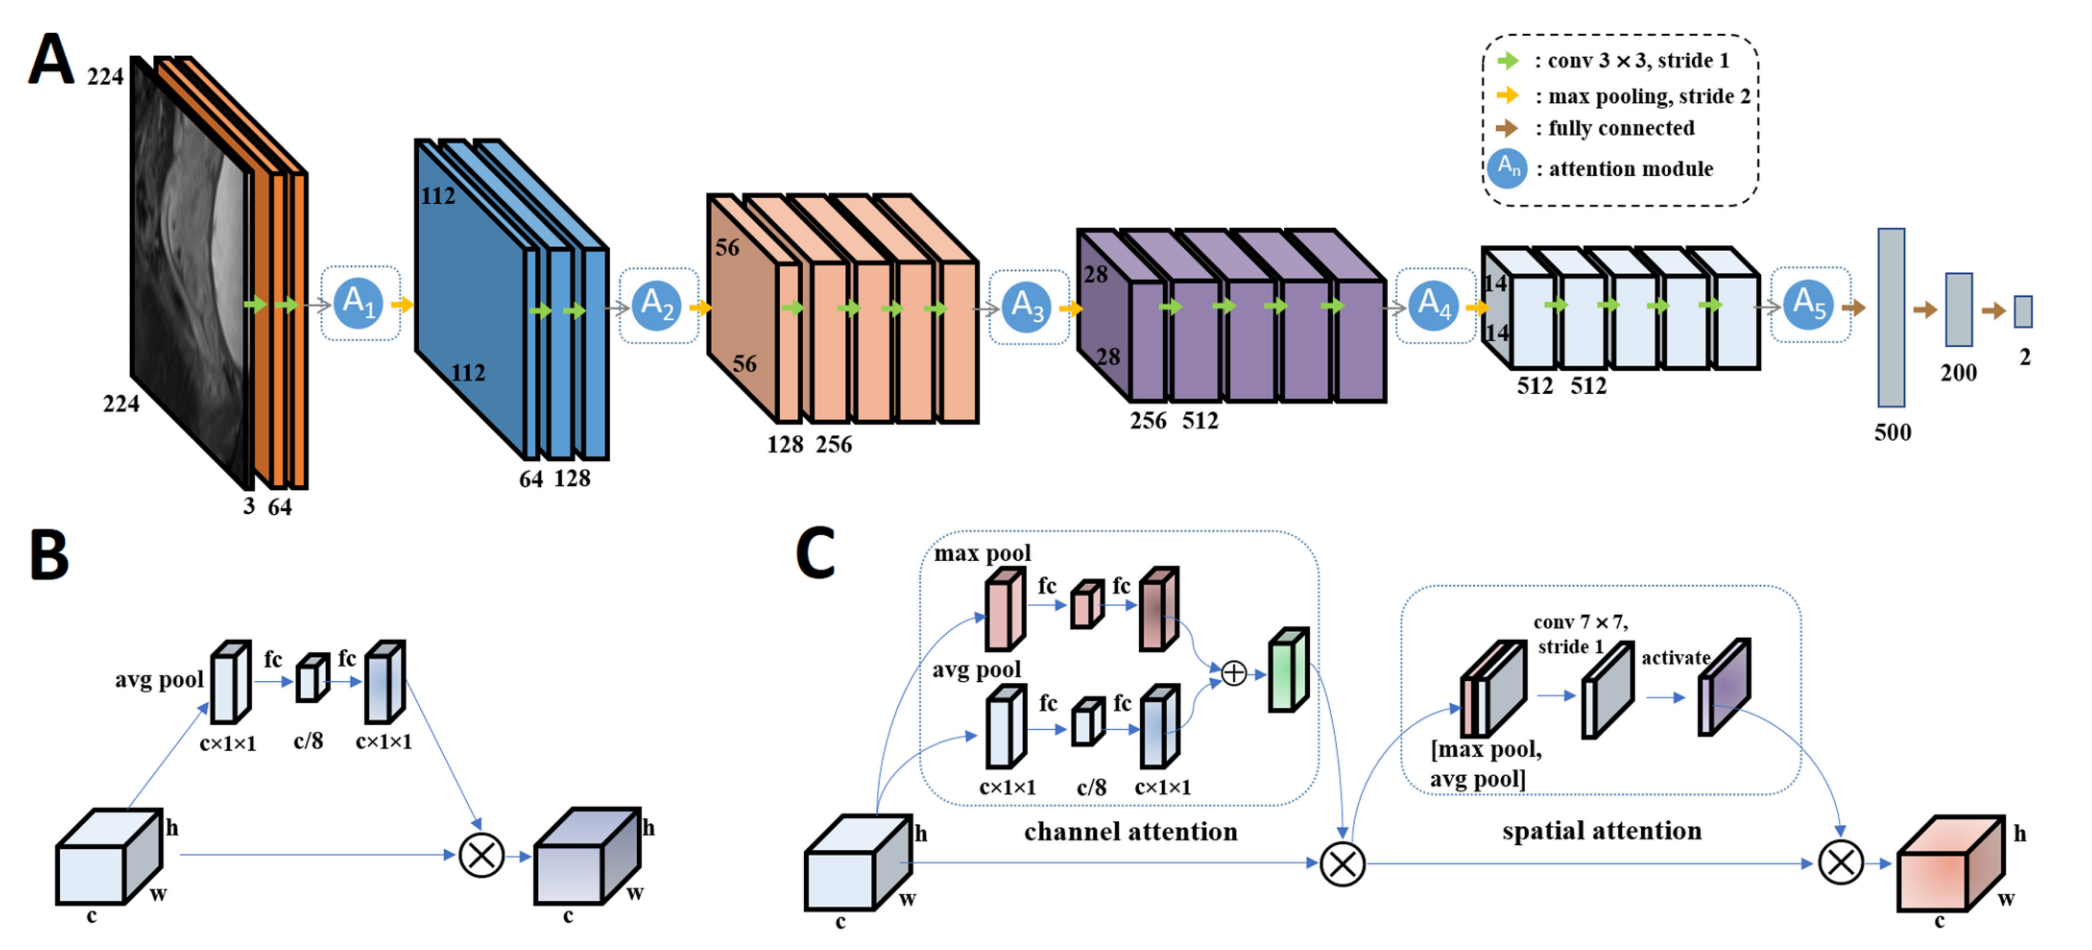
\includegraphics[width=0.8\textwidth]{figures/fig007.png}
    \caption{Fonte: \cite{jiangMRIBasedRadiomics2021}}
    \label{fig:fig007}
\end{figure}

%---------------------------------------------------------
Em outro trabalho, \cite{renBiLSTMMultiheadAttentionbased2023} desenvolveram um modelo avançado usando uma rede Bi-LSTM (memória de longo prazo bidirecional) combinada com um mecanismo de atenção de múltiplas cabeças, utilizando \textit{features} radiômicas e imagens TC de lesões, para aprimorar a diferenciação dos principais subtipos de adenocarcinoma pulmonar, integrando assinaturas radiômicas com características radiológicas de tomografias computadorizadas. O estudo recrutou 421 pacientes de três hospitais, confirmados com adenocarcinoma in situ, adenocarcinoma minimamente invasivo ou adenocarcinoma invasivo, com base na análise de 427 lesões.

A metodologia empregada envolveu a extração de assinaturas radiômicas usando o software `\textit{PyRadiomics}' das regiões de lesões identificadas em cada imagem de tomografia computadorizada. As 100 principais características foram então selecionadas através do método de classificação de características de máxima relevância e mínima redundância. Um modelo preditivo foi subsequentemente desenvolvido empregando essas características juntamente com características radiológicas, usando a estrutura Bi-LSTM e atenção múltipla para classificar as lesões.

O desempenho diagnóstico do modelo foi quantitativamente impressionante, alcançando valores da área sob a curva (AUC) de 0,985, 0,94 e 0,981 nos grupos de treinamento, teste e validação, respectivamente, com precisões correspondentes de 0,92, 0,976 e 0,91. Além disso, comparações foram feitas com dois outros modelos — rede neural convolucional (CNN) + atenção múltipla, e LSTM + atenção múltipla — demonstrando que o modelo Bi-LSTM e atenção múltipla superou essas alternativas em precisão e acurácia no conjunto de testes.

Esta pesquisa destaca a utilidade potente da combinação de técnicas avançadas de aprendizado de máquina com análises radiômicas e radiológicas detalhadas para refinar o processo diagnóstico para subtipos de adenocarcinoma pulmonar, potencialmente orientando abordagens de tratamento mais personalizadas baseadas na caracterização do subtipo.

%---------------------------------------------------------
 \cite{aiSelfAttentionBasedFusion2023} conduziram um estudo inovador intitulado ``Um Modelo de Fusão Baseado em Autoatenção de Características Radiômicas e Profundas para Previsão de Recorrência Precoce em CPNP'', que aborda o significativo desafio de prever a recorrência precoce em câncer de pulmão de células não pequenas usando técnicas avançadas de aprendizado de máquina. Sua pesquisa aproveita o mecanismo de autoatenção para fundir características radiômicas manuais e características de aprendizado profundo extraídas de imagens de TC, com o objetivo de aumentar a precisão preditiva e robustez para recorrência precoce em câncer de pulmão de células não pequenas.

O estudo começou empregando diversas técnicas de aprendizado de máquina para extrair uma variedade de características artesanais de imagens de TC, incluindo atributos de textura, forma e escala de cinza. Para capturar informações semânticas de alto nível e de representação, uma rede ResNet50 pré-treinada foi utilizada para a extração de \textit{features} profundas. Essas características extraídas foram então fundidas com um vetor de características extraído de dados de texturas de imagens radiômicas e unificado usando um módulo de fusão de autoatenção inovador desenvolvido pelos pesquisadores. Este módulo otimiza e pondera o vetor de características fundidas, aproveitando plenamente o mecanismo de autoatenção para melhorar as capacidades de previsão do modelo. A arquitetura pode ser conferida na Figura \ref{fig:fig008}.

Os resultados experimentais, avaliados no conjunto de dados público Cancer Imaging Archive (TCIA), demonstraram que o modelo proposto superou significativamente os métodos existentes na previsão de recorrência precoce. O modelo exibiu melhorias substanciais em precisão de classificação, sensibilidade, especificidade e a área sob a curva (AUC), destacando seu potencial para guiar o tratamento em estágio inicial e melhorar as taxas de sobrevivência para pacientes com câncer de pulmão de células não pequenas.

Este estudo exemplifica a aplicação de técnicas avançadas de aprendizado de máquina em imagens médicas e oncologia, fornecendo um método robusto para a previsão de recorrência precoce que poderia impactar significativamente os resultados clínicos e as estratégias de tratamento em câncer de pulmão.

\begin{figure}[htbp]
    \centering
    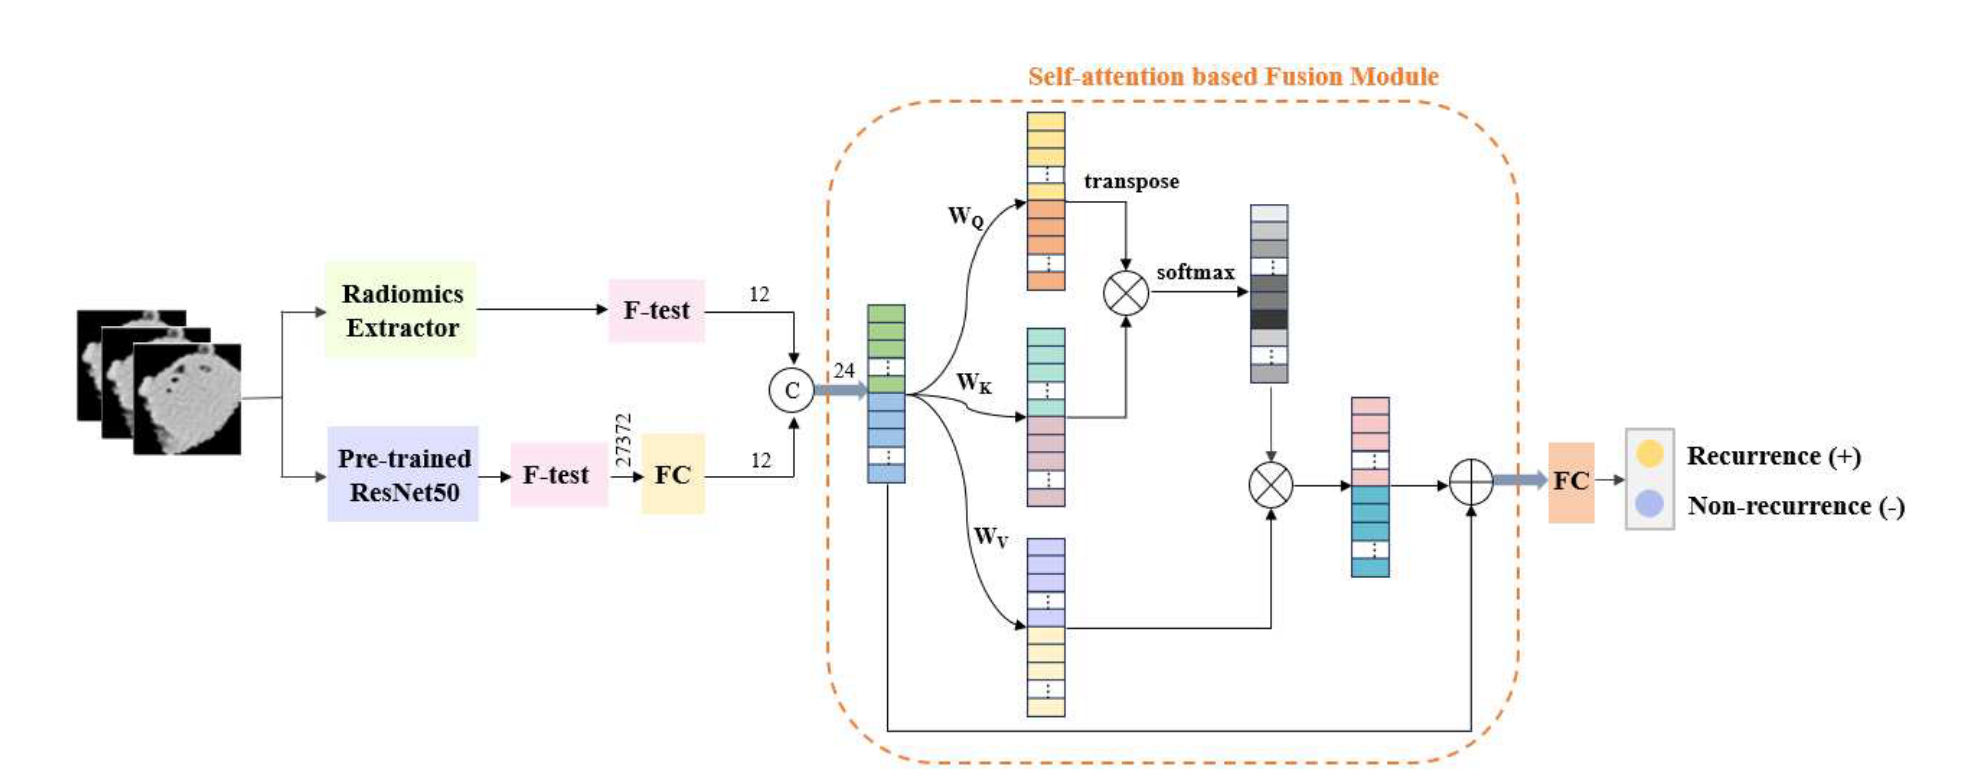
\includegraphics[width=1\textwidth]{figures/fig008.png}
    \caption{Fonte: \cite{aiSelfAttentionBasedFusion2023}}
    \label{fig:fig008}
\end{figure}
%---------------------------------------------------------

\cite{iranmehrImprovedPredictionMGMT2022} desenvolveram uma rede de aprendizado profundo inovadora que utiliza um mecanismo baseado em atenção para aprimorar a previsão do estado de metilação do gene MGMT em glioblastoma muiltifoma (GBM), o tipo mais agressivo de tumor cerebral. Pacientes com GBM possuem uma expectativa muito baixa, entre 18 e 24 meses e requerem tratamentos agressivos, como por exemplo, quimioterapia. Sua pesquisa, apresentada em "Improved Prediction of MGMT Methylation Status in Glioblastoma using a Deep Attention Network", destaca um avanço significativo nas capacidades diagnósticas não invasivas para GBM, que tipicamente tem uma taxa de sobrevivência de apenas 18 meses.

O estudo foca no gene MGMT, cujo estado de metilação é crucial para determinar a eficácia da quimioterapia em pacientes com GBM. As análises radiômicas tradicionais, embora úteis, muitas vezes não capturam os recursos intrincados necessários para uma previsão precisa da metilação. \citeauthor{iranmehrImprovedPredictionMGMT2022} propõem um modelo que integra características radiômicas manuais com técnicas de aprendizado profundo, melhorando a extração de características e a precisão da previsão de GBM.

O modelo introduzido pela equipe utiliza uma combinação de mecanismos de atenção \textit{squeeze} e sequencial para priorizar fatias e regiões relevantes dentro das imagens de ressonância magnética, respectivamente. Esse método não apenas melhora o foco em áreas significativas, mas também aprimora a interpretabilidade geral do modelo. O modelo proposto (Fig. \ref{fig:fig009}) consiste de três etapas: 1) Um modelo base para extrair as \textit{features}, 2) uma rede de atenção temporal e espacial e 3) uma rede de classificação para prever se o exame é metilado ou não metilado. 

\begin{figure}[htbp]
    \centering
    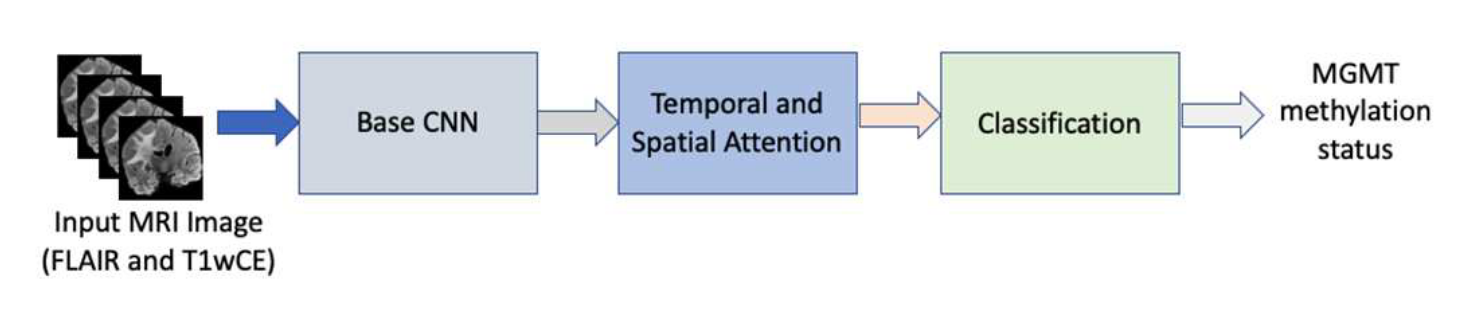
\includegraphics[width=1\textwidth]{figures/fig009.png}
    \caption{Método proposto. \textit{Densenet} foi utilizado como modelo base. A saída da rede densa é alimentada pela rede de atenção que pode priorizar as fatias e regiões. A saída da rede de atenção é enviada à rede de classificação binária para prever o status de metilação do MGMT.}
    \label{fig:fig009}
\end{figure}

O modelo base consiste em uma \textit{DenseNet}. Segundo o autor, a \textit{Densenet} pode suportar milhares de camadas e ser resistente ao \textit{overfitting}. A saída da rede densa é fornecida para a rede de \textit{squeeze} e \textit{self-attention} conforme mostrado na Fig. \ref{fig:fig010}. Cada exame consiste em várias fatias e a \textit{squeeze attention} priorizará as fatias, usando o agrupamento médio global seguido por duas camadas densas separadas e depois o produto escalar com a entrada inicial. A saída da \textit{squeeze attention} é fornecida à rede de \textit{self-attention}. Após a aplicação da \textit{self-attention}, o mapa de atenção contém pixels com uma seção de maior importância em cada fatia. Com a rede de \textit{self-attention}, é possível enfatizar pixels e regiões de diferentes independente da distância em que estes \textit{pixels} se localizam pela imagem. Múltiplas regiões com diferentes tamanhos geradas a partir de regiões integrais são então fornecidas à \textit{attention} sequencial (SA). A rede SA adapta uma rede \textit{long short term memory} (LSTM), que é capaz de aprender dependências de longo prazo. A saída passa por uma camada densa e uma sigmoide para fazer a classificação.

Avaliado em várias métricas de classificação binária, o modelo alcançou a melhor área sob a curva (AUC) de 70,59, demonstrando sua superioridade em relação aos métodos existentes. Este trabalho fornece uma abordagem robusta e automática para capturar características críticas de imagens de ressonância magnética, avançando significativamente na previsão do estado de metilação em GBM em comparação com métodos anteriores. As implicações de tais avanços são profundas, potencialmente melhorando o planejamento de tratamentos personalizados e, em última análise, os resultados para os pacientes com glioblastoma.

\begin{figure}[htbp]
    \centering
    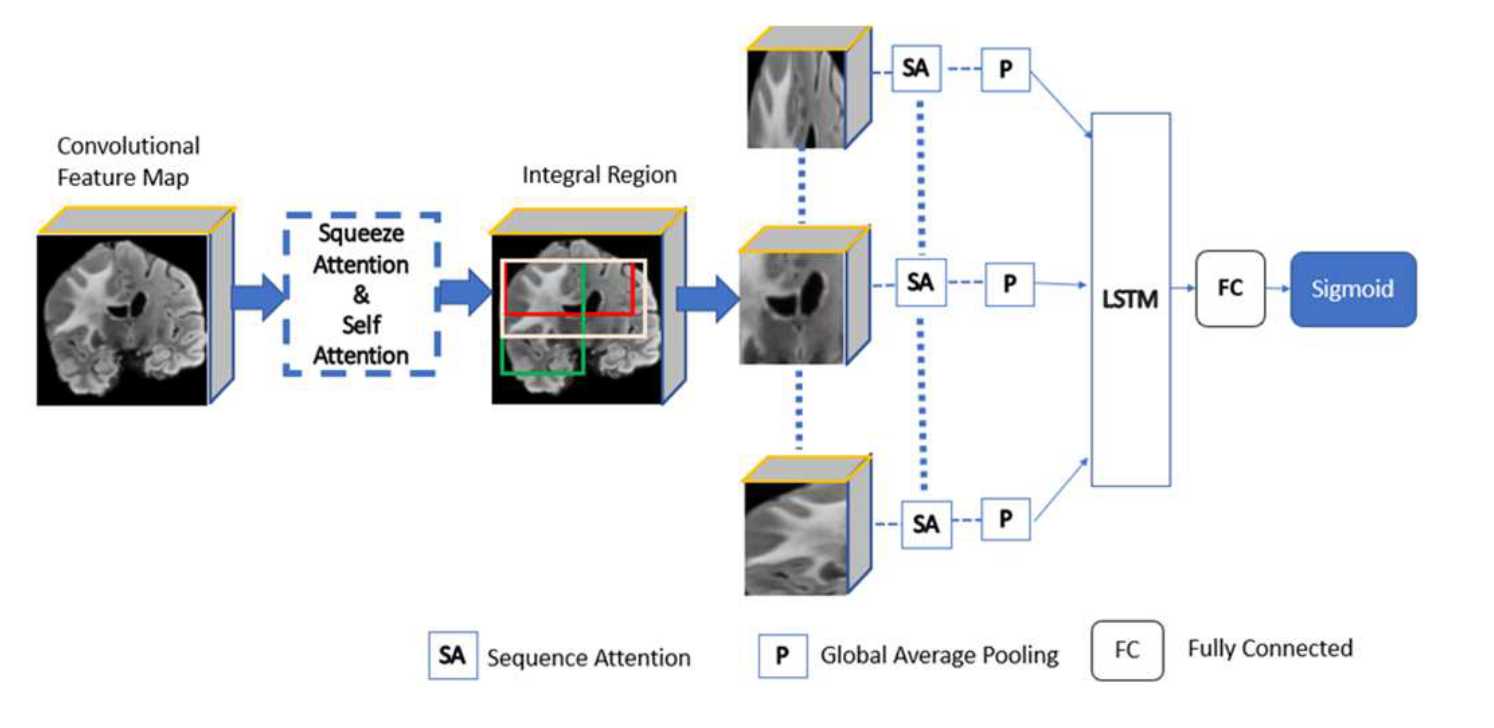
\includegraphics[width=1\textwidth]{figures/fig010.png}
    \caption{Fonte: \cite{iranmehrImprovedPredictionMGMT2022}}
    \label{fig:fig010}
\end{figure}

%---------------------------------------------------------
% \section{Considerações Finais do Capítulo}
% \label{sec:rcond_cap_3}
% \lipsum[2-4]